\documentclass[11pt]{article}
\usepackage[square,numbers]{natbib}
\bibliographystyle{abbrvnat}

% Set margins
\usepackage[margin=2.5cm]{geometry}

% Use Times New Roman or equivalent
\usepackage{mathptmx} % Times New Roman font for text and math

% Set PDF output properties
\usepackage{hyperref} % Optional, for clickable links in the PDF

\usepackage{amsmath}

\usepackage{graphicx}

\graphicspath{
    {figures/}
}


\hypersetup{
    pdfauthor={Dylan Massey}, % Replace with your name
    pdftitle={GNN-based Dialogical Argument Mining}, % Replace with your report title
    pdfsubject={Natural Language Processing}, % Optional, replace with your subject
    pdfkeywords={Argument Mining, Machine Learning, Graph Neural Networks} % Optional, add relevant keywords
}

% Optional: Title setup
\title{GNN-based Dialogical Argument Mining: A First Step} % Replace with your title
\author{Dylan Massey} % Replace with your name
\date{\today} % You can replace \today with a specific date if needed

\begin{document}

\maketitle

\section{Introduction}
\label{sect:intro}

Argument Mining (AM) has established itself as a vital area of research in NLP \citep{stede_argumentation_2019}. Canonically, the task consists of identifying arguments as constellations of propositions, that is: Identifying the propositional content of natural language expressions and subsequently labelling the propositions as being either premise or conclusion (claim) for the a given argument \citep{stede_argumentation_2019}. Further, one is tasked with establishing semantic relations among these propositions. Relations among propositions give rise to argument structures that are \textit{convergent, serial, linked or divergent}\citep{lawrence_argument_2019}. A serial argument, for example, is a chain of propositions where each proposition\footnote{except for the first, which could be considered the \textit{main conclusion}} supports the one that it ``links to". In other cases a proposition might attack another one, only for it to be refuted by a further statement. \\
While considerable efforts have been devoted towards AM on monological argumentative text in written form, \citet{ruiz-dolz_overview_2024} call for attention towards AM of dialogical, spoken data. They organise the \textit{First Task on Dialogical Argument} mining and invite participants to submit AM systems capable classifying relations between propositions, as well as grounding these propositions in locutions through illocutionary force relations, as I discuss in more detail in section \ref{sect:background}. \\
A review of participant contributions allows us to conclude that most systems frame the dialogical argument mining task as a relation identification and classification task. By linearising neighbouring node texts and encoding the text with special tokens the winning team, \citet{binder_dfki-mlst_2024}, achieves 78.78\% on general relation identification between propositional nodes and 55.33\% is achieved in the identification of relations that hold between propositions and their locutionary counterparts. \\
Since the task dataset, compiled by \citet{hautli-janisz_qt30_2022} is graph-structured, in the present paper I ask: Is a GNN-approach, that is, one that is architecturally more assimilated to the task dataset, a viable architecture for the task of dialogical AM?

My main contributions are:
\begin{enumerate}
    \item I am the first to my knowledge to conceptualise the dialogical argument mining (DialAM) task as a node prediction problem.
    \item I provide a first implementation of DialAM using PyTorch Geometric with an evaluation on the performance of the model. Initial results show the challenges of solving the task with a GNN.
\end{enumerate}

\section{Background}
\label{sect:background}

\paragraph{Argument Mining.} The field of argument mining is concerned with eliciting the argument structure of natural language text. This argument structure consists of propositions, which are the most basal units of argumentation along with the relations that hold between them. Such relations can either be \textit{supportive} or \textit{attacking}, or stand in a neutral constellation towards eachother. 

Traditionally the AM task comprises of four subtasks as detailed in \citet{ye_end--end_2021}. The first step consists of determining whether a segment of text is argumentative or not, this is referred to by \citet{ye_end--end_2021} as \textit{component segmentation}. As a second step in the classical argumentation mining pipeline comes the necessity to classify what ``type'' the argumentative text is: Is it a premise or is it a claim? These two subtasts are often referred to as component identification. The next two subtasks are (1) finding out if a relation between two argument component holds, and if yes, what type that relation is. A component might be supportive of another one, especially the central claim or attempt to attack it.

Looking at arguments at a higher level we can identify structures of how the different premises / propositions culminating in a central claim are structured. \citet{stede_argumentation_2019} note that different types can emerge. As explained in section \ref{sect:intro} serial arguments are a chain of propositions where each proposition supports the one that it ``links to". Linked argument structured show that there is a dependency between two permisses in supporting a claim. In the case of convergent arguments there is no such interdependency and the two permisses operate to supporting the claim independently. Divergent arguments are the opposite of convergent arguments. In this case a single premise establishes support for two claims. 

An arguments structure might be determined by the text-type it is found in. On a most broad classification, there is a differentiation between monological arguments and dialogical arguments. While considerable research has been performed on monological argumentation, research on dialogical argumentation is still relatively less well-researched \citep{budzynska_towards_2014}. Also the task within which the present paper is based (cf. section \ref{sect:intro}) is set out to reduce this scarcity. On a more fine-grained levels argumentative text can be found in a variety of text types, such as legal texts, scientific articles, or political debates. Additionally one might distinguish argumentative texts by the setting (i.e., broadcasted tv debates vs. parliamentary debates).

\paragraph{Relation Extraction.} An often chosen approach to argument mining is to frame the task as a relation extraction problem with preceeding a preceding entity detection step. In the AM setting, the goal would then be to first identify the propositional elements of a text and then to to identify pairs of propositions in the text and classify the relation holding between the two.
Since arguments can also be seen as a form of dependency structure, research has been carried out of applying dependency parsing models to the AM task. For example, \citet{ye_end--end_2021} frame the task of argument mining as, (a) a biaffine dependency parsing problem and attempt to solve all four subtasks of of argument mining through a single model end-to-end. 

\paragraph{Graph Neural Networks.} Graph neural networks are a relatively novel technology that has been shown to be effective in a variety of tasks, including node classification, link prediction, and graph classification. 
The basic idea is to learn a representation of each node in the graph by aggregating information from its neighbors. 
This is done by passing messages between nodes in the graph, updating each node's representation based on the messages it receives. 
The process is typically repeated for a fixed number of steps, allowing each node to gather information from nodes at varying distances in the graph. 
The final node representations can then be used for downstream tasks such as node classification.  

\section{Method.}
\label{sect:method}

To give a relatively concise overview of what I attempted, I start by briefly discussing the dataset and evaluation and then continue with giving a formal definition of the task and then finally proceed to describe the architecture of the graph neural network that is implemented.

\paragraph{Dataset.} The underlying dataset setup for the task is the \textit{QT30} dataset \citep{hautli-janisz_qt30_2022}. Consists of transcripts of 30 episodes of the BBC debate-show question time\footnote{\url{https://www.bbc.co.uk/programmes/b006t1q9}} aired between 2020-2021. It is considered the largest corpus of dialogical argumentation to date with comprising of around 280'000 words. Thematically, the debates range from Scottish Independence, to the COVID-19 pandemic, the climate crisis as well as the future of the UK. The data is annotating using the Inference Anchoring Theory annotation standard, which has the ability to capture argument structures grounded in dialogue. The annotation scheme used is based on Inference Anchoring Theory \citep{budzynska_towards_2014}. The debates are segmented into a size deemed meaningful yet manageable for the annotators. These segments are then provided as ``nodesets"". The dataset for training contains 1478 nodesets.

\paragraph{Formal Task Definition.}
The goal of the task is establishing relations between units of dialogue (locutions $L$) and argumentative discourse units (propositions, $P$), as well as establishing relations within these two types of units. Then four relation types exist: 

% \begin{equation}
\begin{flalign}
P_{rel} &:: [P] \rightarrow [P] \\
L_{rel} &:: [L] \rightarrow [L] \\
I_{rel} &:: L \rightarrow P \\
C_{rel} &:: L_{rel} \rightarrow P_{rel}
\end{flalign} \\

$P_{rel}$ can take on values of \textit{\{ inference, conflict, rephrase \}}. $L_{rel}$ can only take on \textit{\{ transition \}} and connects the individual locutions in time (sequence of utterances) along a temporal axis. $I_{rel}$ and $C_{rel}$ can take on the same set of values, since they both possess \textit{illocutionary force}, these are the most comprehensive \textit{\{ asserts, agreeing, arguing, assertive\_questioning, challenging, disagreeing, pure\_questioning, restating, rhetorical\_questioning, default\_illocuting \}}. A more detailed explanation of the meanings of the relations and the meaning of the values they can take can be found in \citet[p. 3294]{hautli-janisz_qt30_2022}. \textbf{For the task, instances of $P$ and $L$ are given and the goal is to approximate the relations that hold between them (apart from $L_{rel}$, which is already given)}. Graphically, this amounts to reconstructing a graph where $P$ and $L$ are nodes and the relations can be interpreted as labelled edges. This is also how the provided QT-30 dataset is structured, since the IAT framework defines its annotation scheme as a graph. Figure \ref{fig:arg_graph} in the appendix shows an example of such a graph. Note that a $P_{rel}$ proposition can support / by substantiated by multiple propositions (convergence) and this they are denoted as multi-argument relations and the same holds for locutions. Thus they are denoted as lists in the relations definitions. \\
\\
The SOTA-performance on the dataset in the global context (predicting both illocutionary and argument relations) was achieved within the context of the \textit{First Task for Dialogical Argument Mining} \citep{ruiz-dolz_overview_2024} by \citet{binder_dfki-mlst_2024} (KnowComp), who first approximate whether a relation holds for two nodes for all relations $P_{rel}, I_{rel}, C_{rel}$. They do this through a process they call ``normalisation''.

% Review of exising approaches, who won etc.

\paragraph{Normalisation.} Of particular significance to solving the task appears a method implemented by several participants \citep{binder_dfki-mlst_2024,chaixanien_pungene_2024}. Instead of assembling the structures end-to-end, they use a normalisation step which re-assembles the (directed) edges of most of graph. The reason this works comes from the observation that (a) the dialogue argument graphs are have a ladder-like shape and secondly that there is a high semantic similarity between ther illocutions and their corresponding propositions, which makes it quite easy to reconstruct such a graph. Both teams opt for a text similarty metric to ground propositions int their locutionary counterpars. to This can be seen in figure \ref{fig:arg_graph} in the appendix. \\
\\
As the second step they then treat assign labels to the determined relations. They do this by treating the task as n-ary relation classification. They linearize the nodes of the graph (nodeset) and ``arguments" (adjacent nodes) of the node to be predicted with special tokens depending on the relation type. To predict $P_{rel}$ they get the $L_{rel}$ pointing to $P_{rel}$ via $C_{rel}$  and then the participants of $L_{rel}$ and encode these with the special tokens. For predicting $C_{rel}$ they also encode the participants of $L_{rel}$, but encode with different tokens than for predicting $P_{rel}$. For predicting $I_{rel}$ simply the participating $L$ is encoded. Noteworthy is that their approach is completely independent of the text on the propositional nodes $P$ and only relies on textual representations in $L$.

\paragraph{Evaluation.} For evaluating the success of systems approximating the different relations performance is assessed on the basis of either only successfully predicted relations (\textit{focussed metric}) or on the basis of successfully predicted relations \textbf{and} the successful prediction of the absence of relations (\textit{global metric}). Additionally, the organisers of the shared task separately evaluate performance of predicting $P_{rel}$ (propositional relations) vs. predicting $I_{rel}$ and  $C_{rel}$ (illocutionary relations). The global results of the shared task participants are given as F1-scores in Table \ref{tab:results}. In the scope of this project I only focus on the \textit{global} evaluation metric, since this is the more realistic setting. In the focussed setting the models that apriori assume a link between all nodes (i.e., are ``overly optimistic'') could gain an advantage over more conservative models. \\

\paragraph{Architecture of the Proposed Approach.} While previous approaches to argument mining appear to have been strongly influenced by the relation extraction paradigm, I propose to frame the task as a \textbf{node prediction} task over graphs\footnote{Although we are really predicting the labels of the edges, one can replace a labelled edge with two new edges and a node that represents the label. This aligns better with the structure of the data in the QT-30 corpus.}. Since the dataset of the task is encoded as a graph, I hypothesize that graph-based learning \textit{might} be the natural choice. As inspiration for the architecture serves the paper by \citet{lin_bertgcn_2021}, who show how BERT-based embeddings can benefit from GNN-based neighbourhood generated embeddings for text classification. In other terms, the approach aims to fuse contextual-word embeddings, with the idea of Graph Convolutional Neural Networks. In particular, I use message passing between nodes so they can benefit from local neighbourhood information in addition to their own embeddings. \textbf{I then add these two information sources with their weighted sum}. This weighting leads to a separate manually chooseable parameter that determined how much contribution is from GNN-representations vs. pure DeBERTa representations. A diagram of the model architecture is shown in Figure \ref{fig:arch_map}. On the left the input data is shown (graph-structure). The triangles indicate a $P$ node, the bars are ``pseudo-nodes" that should represent the actual edge labels of a $P_{rel}$. The squares are ``pseudo-nodes" that represent the edge labels for $I_{rel}$ and $C_{rel}$. In the image the green node is the one which I want to predict a label for, i.e. assign either \textit{inference}, \textit{conflict} or \textit{rephrase} to. Since this pseudo-node natively does not contain any text, I use a special token \verb|[S]| and get the CLS-embeddings for the resulting token\footnote{Similarly I use [YA] to get embeddings for the illocutionary relations and [TA] to encode the transition nodes between $L$ }. Simultaneously to feeding the CLS-embeddings into the model, we also generate neighbourhood representations using graph convolutions using the \verb|GCNConv| layer \footnote{\url{https://pytorch-geometric.readthedocs.io/en/2.5.2/generated/torch_geometric.nn.conv.GCNConv.html}}. We do not add any self-loops and perform two convolution operations (for simplicity, the diagram only shows how neighbourhood information is used from one convolution operation). Finally the softmax is computed for the one-hot encoded correct label. I use the same model for prediction of illocutionary relations and argument relations.

I use Categorical Cross Entropy loss to account for the class imbalance in the dataset. I use the Stochastic Gradient Descent with a learning rate of $10^{-4}$ and a momentum of $0.9$ and do not use any batched training. I train the model for 5 epochs. The underlying model for the contextual word embeddings is \verb|microsoft/deberta-v3-small|.

\begin{figure}
    \centering
    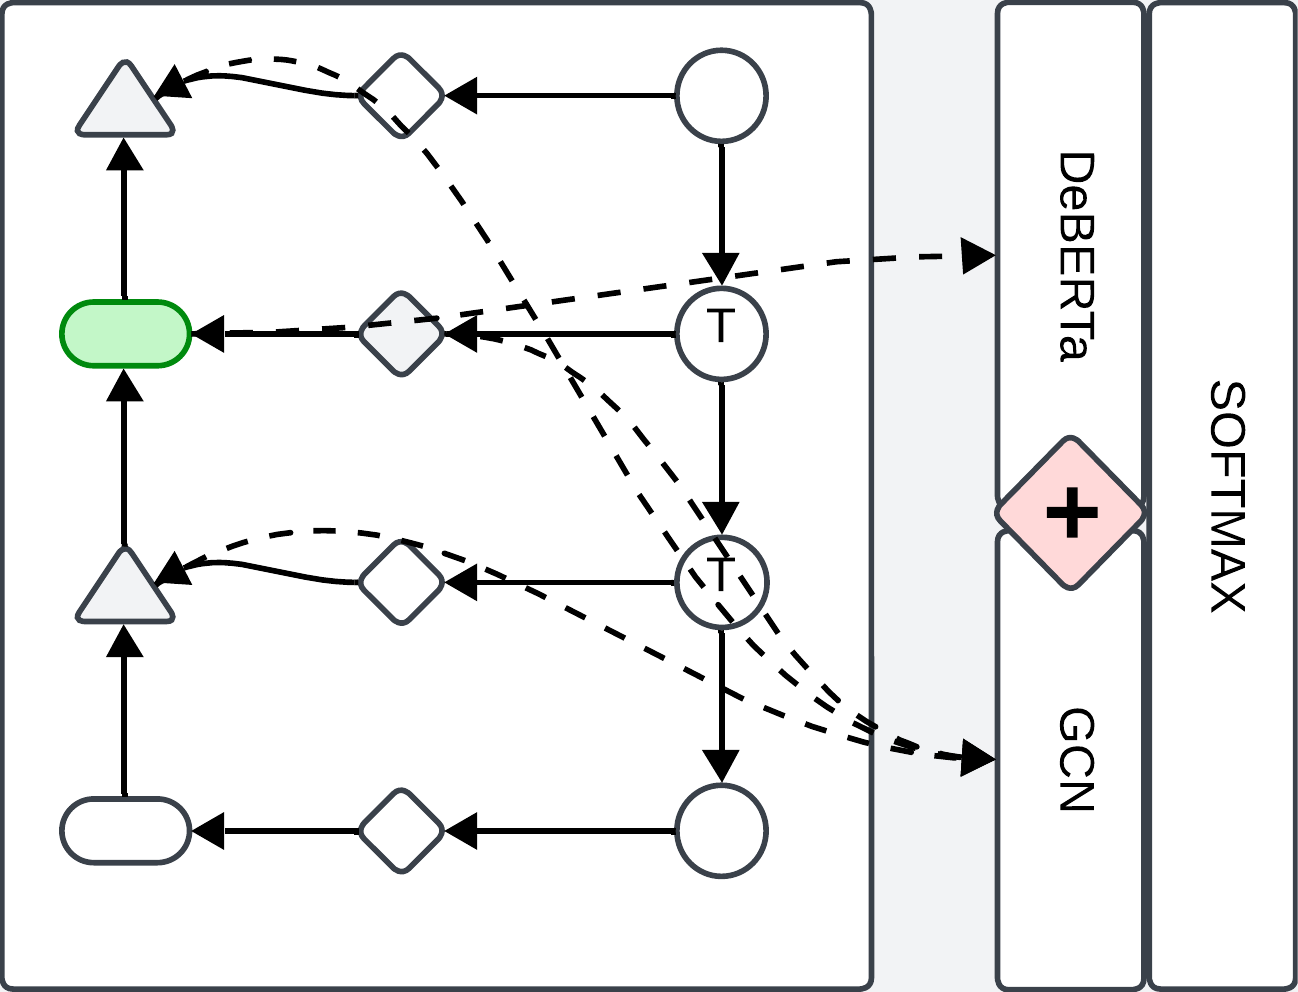
\includegraphics[width=0.5\textwidth]{figures/model_architecture.png}
    \caption{A simplified schema of the proposed implementation.}\label{fig:arch_map}
\end{figure}

% In particular, we use Graph Convolutions.

% What are the benefits of the proposed approach.

% Include image visualisation of model architecture.


\section{Results \& Discussion}

During prototyping it seemed difficult to get any significant learning steps (drop in loss) out of the model. Prototyping was conducted using a small subset (N=20) of the data. Through the feedback during my presentation I was given advice to check how learning would improve by reducing the node predictions to be made to only two labels. Unfortunately, I observed the same problem and the loss did not drop significantly over epochs. What I noticed was that the model has a tendency to consistently predict the same label for all nodes. Naturally this would lead to the conclusion that a class imbalance might be the origin of the problem. Choosing two classes that are approximatively the same size did not lead to any significant improvements, for this test I choose the two classes ``Default Rephrase" (n=71) and ``Restating" (n=64), which are two labels that (a), are structurally positioned differently within the graph and (b) are of similar size. So the discriminative capacity of the model should increase, not last because the pure DeBERTa representation of these nodes is should be easily discernable since different special tokens were used to encode them. Learning however was still problematically slow, which suggested that the presence of a lack of data was not the primary cause of concern for the slow model learning process. Another design choice in GNNs is whether to encode the graph as directed or undirected. The QT-30 nodesets are directed graphs, but in isolating possible variables for the lack of learning in the model I also make the graph symmetric. The learning does not improve / change significantly however. \\
\\
Due to the uncertainty of the origin of the lack of learning of the model (architectural, data-based, problems with data conversion scripts, normalisation). I decided to give the model a go on the full dataset and after training for 5 epochs on all of the 1478 nodesets I found the loss on the training set to have substantially decreased to just $0.004$. The loss on the validation set however stayed high at 1.64 (this is similar to the loss I obtained during experiments on the subset described in the above paragraph. In that case the loss would stay at this ``height'' for training and validation set).  After training, I wanted used an evaluation dataset\footnote{\url{https://github.com/ArneBinder/dialam-2024-shared-task/tree/main/data}} to check the performance of my model, the results however appeared problematic in comparison to the results reported by the task participants. Using the official evaluation script a general score of 67.60 \% was obtained for $ILO_{General}$ F1 and roughly 29.15 \% for $ARI_{General}$ F1. These results are contradictory to the fact that argument relationship identification, that is prediction of $P_{rel}$ is more trivial, since, there are less labels to assign and illocutionary relation identification has a larger set of labels to assign.  \\
Since a GNN with a very similar architecture was used to show benefits of using GNNs for text classification \citep{lin_bertgcn_2021}, it remains unclear why the model does not generalise appropriately to dialogical argument mining. A first step for further diagnosis could be to construct a more trivial taks over a simpler graph structure (that however still pertains to the model architecture) to see sources of potential errors or shortcomings in the model design.

\begin{table}
    % \begin{center}
    \centering
    \setlength{\tabcolsep}{2pt}
    \begin{tabular}{|l|l|l|l|c|c|}
    \hline
    Team name & Task & Paradigm & Model & $\mathrm{ILO}_{\mathrm{General}}\;(\mathrm{F1})$ & $\mathrm{ARI}_{\mathrm{General}}\;(\mathrm{F1})$ \\
    \hline
    DFKI & Rel. Class. & "End-to-end" & DeBERTa & \textbf{55.33} & 78.78 \\
    \hline
    Pungene & Text Class. & Pipelined & BERT-based & 46.22 & \textbf{81.17} \\
    \hline
    Pokemon & Text Class. & Pipelined & De/RoBERTa & 30.64 & 59.36 \\
    \hline
    KnowComp & Rel. Class & Pipelined & DeBERTa & 32.75 & 78.90 \\
    \hline
    Turiya & LLM-based & - & LLaMa & 30.75 & 53.31 \\
    \hline
    \end{tabular}
    \caption{Results on global evaluation for the first task of dialogical argument mining. The most performant team (averaged between ILO and ARI) is DFKI.} \label{tab:results}
% \end{center}
\end{table}

\section{Conclusion}

While the conceptualisation of the dialogical argument mining as node prediction might be novel, the model performance on initial experiments / implementations, do not appear promising. We find a GNN-based approach under the setting we experiment with does not learn well and the performance on the evaluation dataset is not in line with results obtained by other task participants. The model does not seem to be able to learn the task well, which suggests that the model architecture might not be well-suited for the task.

Further investigations of potential technical issues, such as data conversion scripts, normalisation, or the model architecture are needed.

% Similarity to discourse graphs
% https://research.protocol.ai/blog/2023/discourse-graphs-and-the-future-of-science/

% Bibliography (if needed)
%\begin{thebibliography}{9}
%\bibitem{ref1} Author, \textit{Title}, Publisher, Year.
%\end{thebibliography}

\bibliography{references_synced}

\section{Appendix}

\subsection{Argument Graph Example}
\begin{figure}
    \centering
    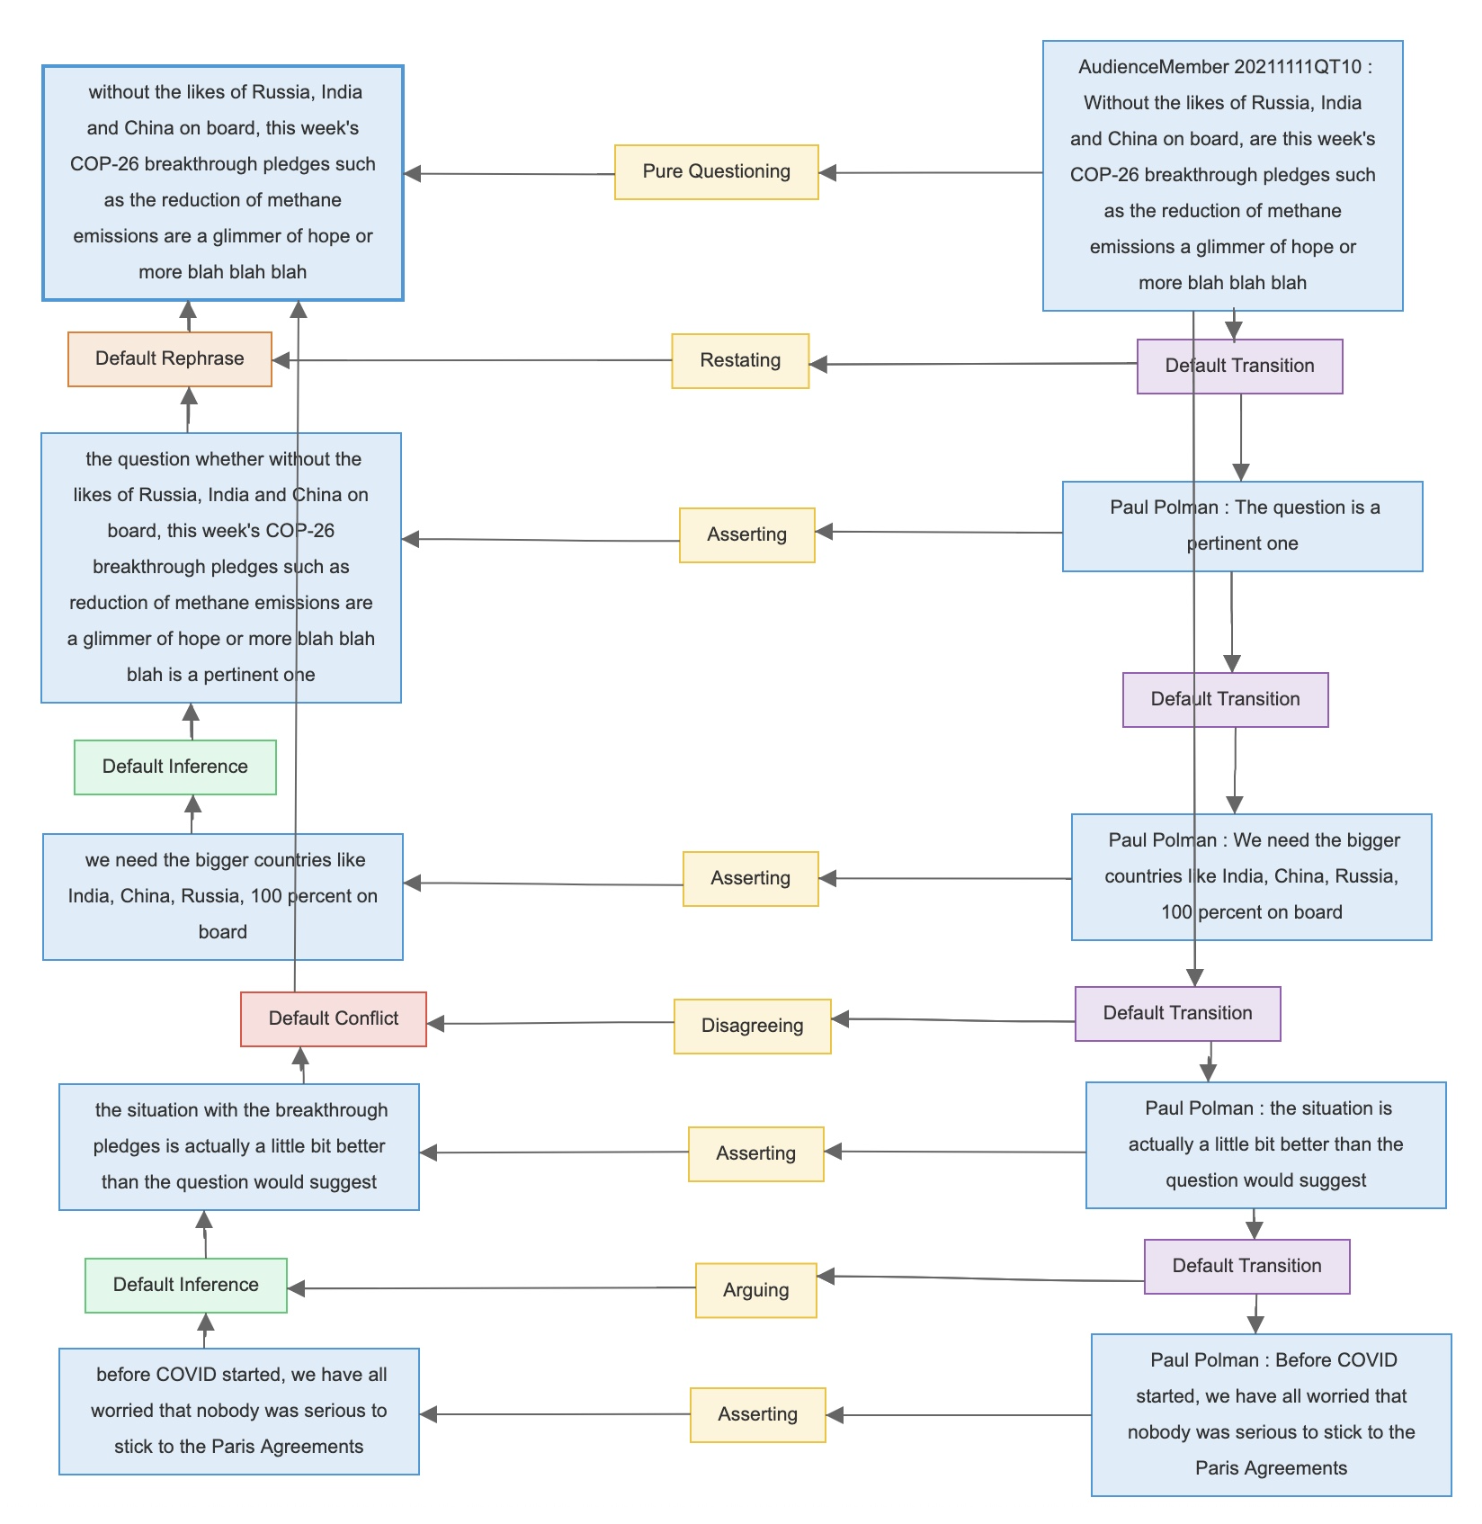
\includegraphics[width=1.0\textwidth]{figures/argument_map.png}
    \caption{An example of an argument graph.}\label{fig:arg_graph}
\end{figure}

\end{document}